\section{压缩映射与不动点}
\label{sec:metric-contraction}

章首的迭代$x^{(t+1)}=x^{(t)}/2+1$想求的是方程$x=x/2+1$的解。很多方程都可以写成$x=T(x)$的形式，再从一个初值出发反复应用$T$。本节把前面的工具用在同一个构造问题上：距离控制给出误差的几何衰减，柯西列与完备性给出极限的存在，连续性验证极限确实是解。然后讨论迭代应在何时停止，以及每步计算有误差时结论怎样修改。本节用带括号的上标$x^{(t)}$表示第$t$次迭代的结果。

\subsection{压缩映射定理}
\label{sec:metric-contraction-theorem}

满足$T(x^\star)=x^\star$的点$x^\star$称为$T$的\term{不动点}（fixed point）。迭代能否找到不动点，取决于$T$是否一致地拉近任意两点。

\begin{definition}[压缩映射]
\label{def:metric-contraction}
设$(X,d)$是度量空间，$T:X\to X$。若存在常数$0\leq q<1$，使所有$x,y\in X$都满足$d(T(x),T(y))\leq q\,d(x,y)$，就称$T$为\term{压缩映射}（contraction mapping），$q$称为压缩常数。
\end{definition}

压缩映射是Lipschitz常数小于$1$的自映射：它把$X$映回$X$自身，所以迭代可以无限进行下去；它对所有点对使用同一个$q$，所以每一步都至少把距离缩小到原来的$q$倍。

\begin{theorem}[压缩映射定理]
\label{thm:metric-contraction}
设$(X,d)$是非空完备度量空间，$T:X\to X$是压缩常数为$q$的压缩映射。则$T$有唯一的不动点$x^\star$，并且对任意初值$x^{(0)}\in X$，迭代$x^{(t+1)}=T(x^{(t)})$收敛到$x^\star$。
\end{theorem}

\begin{proof}
\emph{相邻差几何衰减。}由压缩条件，
\[
  d(x^{(t+1)},x^{(t)})=d\bigl(T(x^{(t)}),T(x^{(t-1)})\bigr)\leq q\,d(x^{(t)},x^{(t-1)}),
\]
反复使用得到$d(x^{(t+1)},x^{(t)})\leq q^t\,d(x^{(1)},x^{(0)})$。

\emph{迭代列是柯西列。}对$s>t$，沿中间各项用三角不等式，再对几何级数求和：
\begin{equation}
\label{eq:metric-contraction-tail}
  \begin{aligned}
    d(x^{(s)},x^{(t)})&\leq\sum_{k=t}^{s-1}d(x^{(k+1)},x^{(k)})
    \leq\sum_{k=t}^{s-1}q^k\,d(x^{(1)},x^{(0)})\\
    &\leq\frac{q^t}{1-q}\,d(x^{(1)},x^{(0)}).
  \end{aligned}
\end{equation}
因为$0\leq q<1$，右边在$t\to\infty$时趋于零，且与$s$无关，所以$(x^{(t)})$是柯西列。

\emph{极限存在且是不动点。}$X$完备，所以存在$x^\star\in X$使$x^{(t)}\to x^\star$。压缩映射是Lipschitz映射，因而连续，由序列判据$T(x^{(t)})\to T(x^\star)$。而$T(x^{(t)})=x^{(t+1)}\to x^\star$，由极限唯一，$T(x^\star)=x^\star$。

\emph{唯一性。}若$T(y^\star)=y^\star$，则$d(x^\star,y^\star)=d(T(x^\star),T(y^\star))\leq q\,d(x^\star,y^\star)$，即$(1-q)\,d(x^\star,y^\star)\leq0$。由$q<1$，$d(x^\star,y^\star)=0$，$x^\star=y^\star$。
\end{proof}

对$T(x)=x/2+1$，在$\mathbb R$上$|T(x)-T(y)|=|x-y|/2$，$q=1/2$，$\mathbb R$完备，所以有唯一不动点；解$x=x/2+1$得$x^\star=2$。从$x^{(0)}=0$出发，迭代依次为$0,\ 1,\ 1.5,\ 1.75,\ 1.875,\ 1.9375,\dots$，误差$|x^{(t)}-2|=2^{1-t}$每步减半。图~\ref{fig:metric-contraction}(a)用蛛网图画出了这个过程：在$y=T(x)$与$y=x$之间来回走折线，折线逐步收拢到两线的交点。

\paragraph{各条件的职责}
定理的四个条件各有作用，缺一不可。非空保证有初值可取。自映射保证每次迭代都留在$X$中。完备性提供极限：$T(x)=x/2$作为$(0,1)\to(0,1)$的映射满足$q=1/2$，迭代$x^{(t)}=2^{-t}x^{(0)}$是柯西列，但它在$\mathbb R$中的极限$0$不在$(0,1)$中，$T$在$(0,1)$上没有不动点。统一的$q<1$提供几何衰减：平移$T(x)=x+1$满足$|T(x)-T(y)|=|x-y|$，常数等于$1$，在完备的$\mathbb R$上却没有不动点。仅仅“相邻距离逐渐变小”也不够：$x^{(t)}=\sum_{k=1}^t1/k$的相邻差$1/(t+1)$趋于零，点列却趋于无穷，因为相邻差之和发散；压缩条件保证的是相邻差按几何级数衰减，其和有限。

\subsection{迭代误差与停止条件}
\label{sec:metric-contraction-error}

实际计算只能进行有限步，需要在不知道$x^\star$的情况下判断当前结果有多准确。证明中的几何尾和给出了答案。

\paragraph{先验与后验误差界}
在式~\eqref{eq:metric-contraction-tail}中令$s\to\infty$。由$d(\cdot,x^{(t)})$的连续性，左边趋于$d(x^\star,x^{(t)})$，于是得到\term{先验误差界}（a priori error bound）
\begin{equation}
\label{eq:metric-a-priori}
  d(x^{(t)},x^\star)\leq\frac{q^t}{1-q}\,d(x^{(1)},x^{(0)}).
\end{equation}
它只用第一步的位移，迭代开始前就能算出达到给定精度所需的步数。若把第$t-1$步看作新的初值，同一个估计给出$d(x^{(t)},x^\star)\leq\dfrac{q}{1-q}\,d(x^{(t)},x^{(t-1)})$，称为\term{后验误差界}（a posteriori error bound）
\begin{equation}
\label{eq:metric-a-posteriori}
  d(x^{(t)},x^\star)\leq\frac{q}{1-q}\,d(x^{(t)},x^{(t-1)}).
\end{equation}
它使用当前的相邻差，迭代过程中可以随时检查。

\begin{example}[按目标精度停止]
\label{ex:metric-contraction-stop}
对$T(x)=x/2+1$、$x^{(0)}=0$，有$q=1/2$、$d(x^{(1)},x^{(0)})=1$，先验界为$2^{1-t}$。要求误差不超过$10^{-3}$，需要$2^{t-1}\geq1000$；由$2^9=512<1000\leq1024=2^{10}$，取$t=11$，此时$x^{(11)}=1.9990234375$，误差$2^{-10}\approx0.000977$。后验界的系数$q/(1-q)=1$，例如$t=5$时$d(x^{(5)},x^{(4)})=1.9375-1.875=0.0625$，后验界为$0.0625$，而实际误差$|1.9375-2|=0.0625$。这个线性例子中两个误差界都恰好取等号。
\end{example}

\paragraph{收缩缓慢时的停止判断}
后验界中的系数$q/(1-q)$在$q$接近$1$时很大，小的相邻差可能对应大的误差。取$T(x)=0.99x+1$，它在$\mathbb R$上是$q=0.99$的压缩映射，不动点为$x^\star=100$。从$x^{(0)}=0$出发，$x^{(t)}=100(1-0.99^t)$，相邻差$d(x^{(t+1)},x^{(t)})=0.99^t$。当$t=459$时相邻差约为$0.00992$，首次小于$0.01$；而此时$x^{(460)}$的误差$100\cdot0.99^{460}\approx0.982$，几乎是相邻差的$99$倍，与后验界一致。若只凭“相邻两次变化小于$0.01$”就停止，结果会差将近$1$。先验界$100\cdot0.99^t\leq10^{-3}$要求$t\geq\ln(10^{-5})/\ln0.99\approx1145.5$，即约$1146$步，而$q=1/2$时只需$11$步。两个例子都满足定理的全部条件，定理保证收敛，却不保证收敛得快。

\subsection{带误差的压缩迭代}
\label{sec:metric-inexact-contraction}

实际计算中，$T(x^{(t)})$往往只能近似求出，例如受浮点舍入或内层迭代截断的影响。设精确映射$T$仍满足压缩条件，而实际得到的$x^{(t+1)}\in X$满足
\[
  d(x^{(t+1)},T(x^{(t)}))\leq\eta_t,
\]
其中$\eta_t\geq0$是第$t$步的执行误差。近似点必须仍在$X$中，否则压缩条件无从使用。

\paragraph{误差递推}
令$e_t=d(x^{(t)},x^\star)$。由三角不等式与$T(x^\star)=x^\star$，
\[
  e_{t+1}\leq d(x^{(t+1)},T(x^{(t)}))+d(T(x^{(t)}),T(x^\star))\leq\eta_t+q\,e_t.
\]
反复代入得到
\begin{equation}
\label{eq:metric-inexact-error}
  e_t\leq q^t e_0+\sum_{s=0}^{t-1}q^{t-1-s}\eta_s.
\end{equation}
第一项是初始误差的几何衰减，与精确迭代相同；第二项是各步新引入的误差，它们被后续步骤按$q$的幂次逐渐压缩，但不会消失。

\begin{theorem}[带误差的压缩迭代]
\label{thm:metric-inexact-contraction}
在上述设定下：(1) 若$\eta_t\leq\eta$对所有$t$成立，则$e_t\leq q^te_0+\eta/(1-q)$，从而$\limsup_{t\to\infty}e_t\leq\eta/(1-q)$；(2) 若$\eta_t\to0$，则$e_t\to0$，即$x^{(t)}\to x^\star$。
\end{theorem}

\begin{proof}
(1) 在式~\eqref{eq:metric-inexact-error}中把每个$\eta_s$放大为$\eta$，得到$\sum_{s=0}^{t-1}q^{t-1-s}\eta\leq\eta\sum_{k=0}^\infty q^k=\eta/(1-q)$。再令$t\to\infty$，$q^te_0\to0$。

(2) 设$\varepsilon>0$，取$S$使$s\geq S$时$\eta_s<\varepsilon$。对$t>S$，把和式分成$s<S$与$s\geq S$两段：
\[
  \sum_{s=0}^{t-1}q^{t-1-s}\eta_s
  \leq q^{t-S}\sum_{s=0}^{S-1}\eta_s+\varepsilon\sum_{k=0}^{\infty}q^k
  =q^{t-S}\sum_{s=0}^{S-1}\eta_s+\frac{\varepsilon}{1-q},
\]
其中第一段用了$s<S$时$q^{t-1-s}\leq q^{t-S}$。$S$固定后，第一项在$t\to\infty$时趋于零，所以$\limsup_te_t\leq\varepsilon/(1-q)$。$\varepsilon$任意，故$e_t\to0$。
\end{proof}

\begin{example}[固定执行误差]
\label{ex:metric-inexact-example}
对$T(x)=x/2+1$，设每步实际计算$x^{(t+1)}=T(x^{(t)})+0.1$，即$\eta_t=0.1$。从$x^{(0)}=0$出发，迭代依次为$0,\ 1.1,\ 1.65,\ 1.925,\ 2.0625,\ 2.13125,\dots$，收敛到$x/2+1.1=x$的解$2.2$，与精确不动点$2$相差$0.2$。定理~\ref{thm:metric-inexact-contraction}(1)给出的界$\eta/(1-q)=0.1/(1/2)=0.2$在这里恰好达到。图~\ref{fig:metric-contraction}(b)比较了精确迭代与带误差迭代的误差：前者每步减半，后者先下降，再停在$0.2$附近。
\end{example}

\begin{figure*}[!htbp]
  \centering
  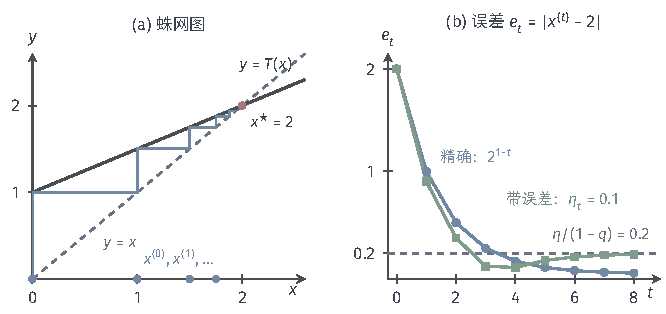
\includegraphics[width=112.691mm]{figures/02-abstract-mathematics/01-metric-and-measure/tikz/c1-contraction/figure.pdf}
  \caption{压缩迭代$T(x)=x/2+1$，初值$x^{(0)}=0$。(a) 蛛网图：从$x^{(0)}$出发竖直走到曲线$y=T(x)$，再水平走到对角线$y=x$，得到下一个迭代值；折线收拢到交点$x^\star=2$。(b) 误差$e_t=|x^{(t)}-2|$：蓝色为精确迭代，$e_t=2^{1-t}$；绿色为每步加入执行误差$0.1$的迭代，误差先下降，越过精确解后趋向$0.2$；灰色虚线是误差上界$\eta/(1-q)=0.2$。}
  \label{fig:metric-contraction}
\end{figure*}

\paragraph{带误差时的停止判断}
执行误差也改变停止判断。对任意$x\in X$，$d(x,x^\star)\leq d(x,T(x))+d(T(x),T(x^\star))\leq d(x,T(x))+q\,d(x,x^\star)$，所以$d(x,x^\star)\leq d(x,T(x))/(1-q)$。取$x=x^{(t)}$，并用$d(x^{(t)},T(x^{(t)}))\leq d(x^{(t)},x^{(t+1)})+\eta_t$，得到
\[
  e_t\leq\frac{d(x^{(t+1)},x^{(t)})+\eta_t}{1-q}.
\]
可观测的相邻差必须连同本步执行误差一起判断：在上例中，迭代停在$2.2$附近时相邻差趋于零，但$\eta_t=0.1$使右边始终不小于$0.2$，正确地提示结果并没有比$0.2$更准。本节只保留这一通用机制；线性方程组的迭代解法和最优化中的迭代算法，会在相应部分利用具体结构给出压缩常数。
